\documentclass[../main.tex]{subfiles}

\begin{document}

Neuronale Netzwerke können als Implementierung eines Gehirns auf einem Computer verstanden werden. Die Funktionsweise eines Neuronalen Netzwerkes wurde vom biologischen Vorbild abgeschaut und an die Gegebenheiten eines Computers angepasst. 

Der größte Unterschied zwischen der klassischen Programmierung und der Erstellung von Neuronalen Netzwerken ist, dass bei der Erstellung eines Netzwerkes nicht die tatsächlichen Berechnungen festgelegt werden, sondern diese mit Trainingsdatensätze erst gelernt werden müssen. Der Softwareentwickler kann lediglich an Paramentern drehen und beispielsweise die Anzahl der Neuronen oder die Anzahl der Layer eines Netzwerkes festlegen.
Große Firmen wie Google, Facebook oder Apple sammeln hierfür schon seit Jahren Daten von Nutzern, um diese für das Trainieren von Netzwerken zu verwenden und dadurch neue Geschäftsmodelle zu entwickeln.

\section{Funktionsweise Perceptron}
Die Idee der Perceptrons wurde von Frank Rosenblatt das erste mal 1958 in einem Paper erläutert (\cite{paperPerceptron}). Der Unterschied zu noch älteren Modellen war, dass sich die Struktur eines Netzes beim Modell von Rosenblatt nicht während des Lernens ändert, sondern sich nur die Schwellwerte der einzelnen Perzeptronen ändern. Zuvor wurde versucht, den Lernvorgang eines biologischen Gehirns möglichst genau auf dem PC zu Implementieren. Später wurde das Modell von Minsky und Papert untersucht und vereinfacht. (\cite{articleTheorieDerNeuronalenNetze})

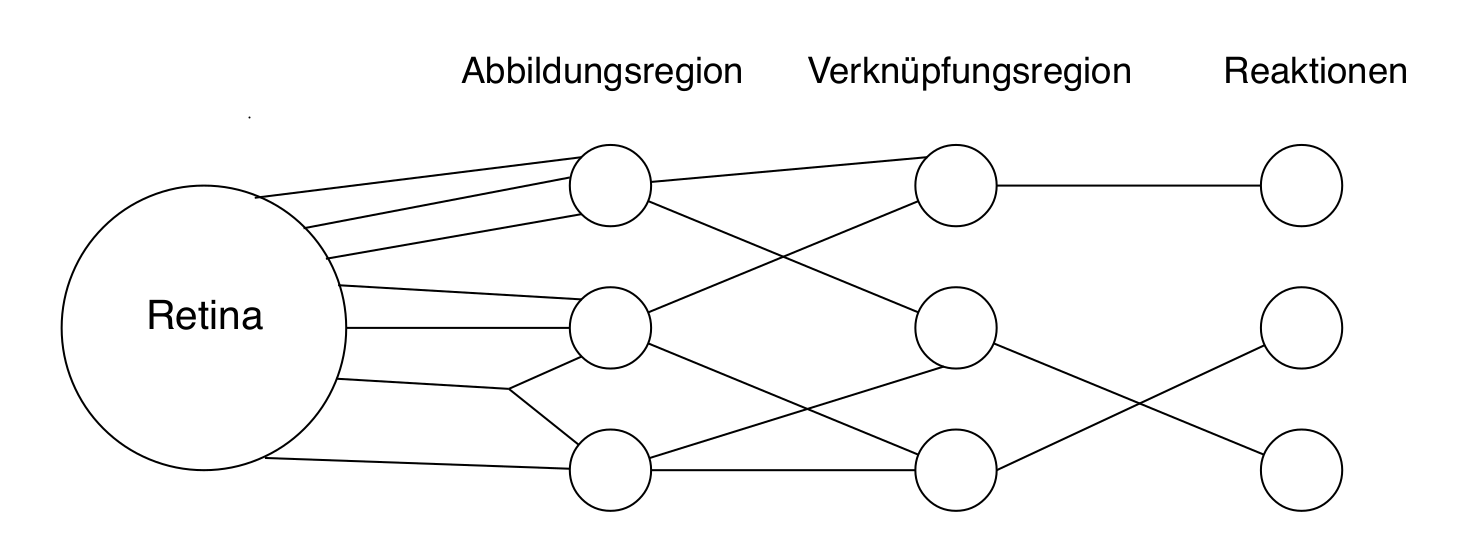
\includegraphics[width=\textwidth]{../images/Benz/Netz_Perceptron.png}

Die Grafik zeigt ein Netz mit Perzeptronen nach Rosenblatt. Auf die Retina, dem Fachbegriff für die biologische Netzhaut eines Auges, wird ein Bild abgebildet. Die Retinapunkte sind mit der ersten Schicht von Perceptronen fest, deterministisch verbunden. Die Verbindungen zur zweiten Schicht, der Verknüpfungsschicht, sind zufällig gewählt. Ebenso sind auch die Verbindungen zwischen der zweiten und der dritten Schicht zufällig gewählt.

"Die Idee von Rosenblatt war, mit der Verknüpfungsregion bestimmte Muster in der Eingabe aus den Retinapunkten zu erkennen und die entsprechende Reaktion zu steuern. Der Lernalgorithmus muß die notwendigen Gewichte finden, um Muster aus der Retina mit Reaktionen zu assoziieren. (\cite{articleTheorieDerNeuronalenNetze})"

Das Modell von Rosenblatt wurde im Lauf der Zeit immer weiter reduzier. Wird heute von Perceptronen gesprochen, besitzen diese mehrere binäre Inputs und einen binären Output. (\cite{neuralNetworksAndDeepLearning}) In der Grafik unterhalb hat das Perceptron $3$ Inputs, es kann aber ebenso weniger oder mehr Inputs besitzen.

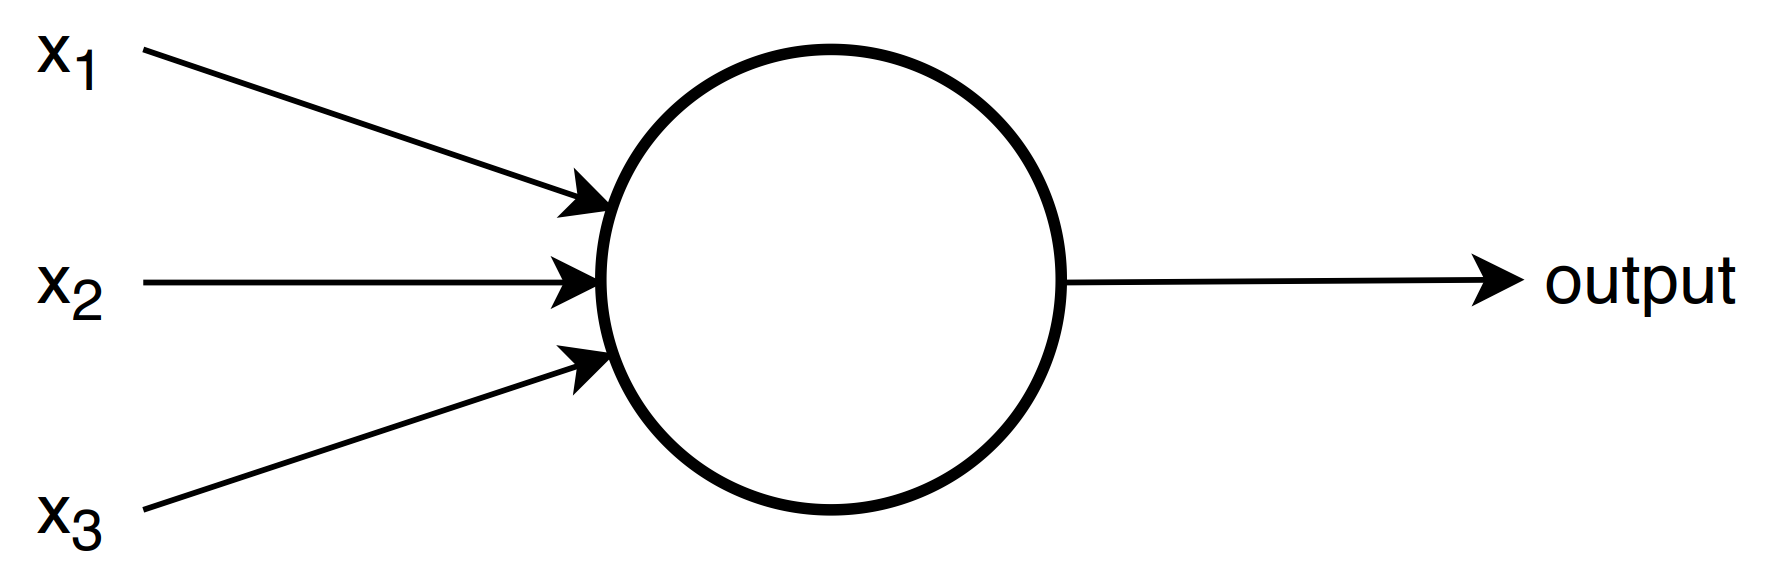
\includegraphics[width=0.7\textwidth, center]{../images/Benz/perceptron.png}

Der Wert des Outputs ist abhängig von den Werte der Inputs. Rosenblatt führte für die Inputs Gewichte ein. Für jeden Input \(x_{j}\) gibt es ein bestimmtes Gewicht \(w_{j}\) aus dem Menge der natürlichen Zahlen. Ist die Summer der Multiplikation von Input mit dazugehörigem Gewicht größer als ein Schwellwert, ist der Output $1$. Ist die Summer kleiner als der Schwellwert, ist der Output $0$.

\begin{align}
	output &= \left \{ \begin{matrix}
	0 \qquad falls \quad \sum_{j} x_{j}*w_{j} \leq Schwellwert \\ 
	1 \qquad falls \quad \sum_{j} x_{j}*w_{j} > Schwellwert
	\end{matrix} \right.
\end{align}

Mit den Funktionen des Perceptrons können schon einfache Problemstellungen logisch gelöst werden. Außerdem können mit diesen Perceptronen logische Gatterschaltungen entworfen werden, da sie sich ähnlich wie digitale Bausteine verhalten. \cite{neuralNetworksAndDeepLearning}

Für schwierigere Probleme, wie die Erkennung von handgeschriebenen Ziffern, sind die Perceptronen jedoch nicht mächtig genug und nur sehr eingeschränkt benutzbar. Ein weiterer Nachteil der Perceptonen ist, dass ein Netzwerk, aufgrund der verwendeten natürlichen Zahlen, nur schwer trainierbar ist. Deswegen werden heute für Neuronale Netzwerke andere Neuronen verwendet, die Grundidee dahinter ist jedoch auch nach 60 Jahren noch die gleiche.

\addtocontents{toc}{~\hfill B. Riedle\par}
\section{Aktivierungen}
Perceptronen bieten in ihrer Grundform die Möglichkeit, unbeschränkte Eingaben mit unbeschränkten Gewichten und zu verarbeiten. Ihre Ausgabe wiederum ist bekanntlich auf die diskreten Werte $1$ oder $0$ beschränkt. Um es Perceptronen zu ermöglichen, ein lernendes Netzwerk aufzubauen, ist es notwendig, dafür zu sorgen, dass die Ausgaben der Perceptronen beherrschbar bleiben. Ziel ist es, mit kleinen Veränderungen der Gewichte und Biases auch kleine Veränderungen der Outputs zu bewirken (vgl. \cite{NNADL_sigmoid_1}). Bei Verwendung der klassischen Perceptronen können kleine Änderungen der Weights $w$ und Biases $b$ nur Änderungen in der Ausgabe in Form von Sprüngen zwischen $0$ und $1$ und vice versa bewirken. \par
Um nun auch kleine Änderungen in den Outputs eines Perceptrons zu gestatten, wird die Funktion zur Bestimmung dessen nach Gleichung \ref{eq:output_1} zu \ref{eq:output_2}] modifiziert. 
\begin{align}\label{eq:output_1}
	output &= \left \{ \begin{matrix}
	0 \qquad falls \quad w \cdot x + b \leq 0 \\ 1 \qquad falls \quad w\cdot x + b > 0
	\end{matrix} \right . \\\label{eq:output_2}
	output &= a(w\cdot x + b) 
\end{align}
Hierbei stellt $a(x)$ eine sogenannte Aktivierungsfunktion dar. Aufgabe dieser Funktion ist es, die erzeugte Ausgabe kontinuierlich im Intervall $[0;1]$ zu verteilen. \\ Damit ist gewährleistet, dass kleine Änderungen in Weights und Biases auch kleine Änderungen in den Outputs der Neuronen erzeugen. Es existieren einige geeignete Aktivierungsfunktionen, die die genannten Eigenschaften besitzen. In der Praxis werden auch verschiedene solcher Funktionen verwendet. Durch geschickte Wahl der Aktivierungsfunkton kann das Verhalten des Netzes für die entsprechende Aufgabe optimiert werden.\\ In dieser Arbeit wurden zwei unterschiedliche Aktivierungsfunktionen genutzt. Diese sollen im folgenden kurz dargestellt werden. \paragraph{Sigmoidfunktion} 
Die Sigmoidfunktion $\sigma(x)$ enstpricht den gegebenen Forderungen an eine Aktivierungsfunktion $a(x)$ und bildet damit den Definitionsbereich $\mathbb{D} = ]-\infty; \infty [$ auf den Wertebereich $\mathbb{W} = ]0;1[$ ab. Der Begriff Sigmoidfunktion wird hier wie auch häufig an anderer Stelle für den Spezialfall der \emph{logistischen Funktion} verwendet, welche nach Gleichung \ref{eq:sigmoid_function} definiert wird.
\begin{align}
	\sigma(x) = \frac{1}{1 + e^{-x}} \label{eq:sigmoid_function}
\end{align}
Im Fall der Neuronalen Netze wird die Sigmoidfunktion $\sigma(x)$ auf das Ergebnis der Operation $w\cdot x + b$ angewandt. Damit bestimmt sich also der Output der Perceptronen nach Gleichung \ref{eq:sigmoid_perceptron}. 
\begin{align} %\label{eq:sigmoid_perceptron}
	output = %\simga(w\cdot x + b) = \frac{1}{1 + e^{-(w\cdot x + b)}} 
\end{align}
Nachteile dieser Funktion sind die schnelle Annäherung der Funktion an die Endwerte $0$ und $1$, sowie ihr Nulldurchgang bei $0.5$. Sie ist daher nur für betragsmäßig kleine Gewichte $w$ und Biases $b$ geeignet. Ihr Graph ist in Abbildung \ref{fig:sigmoid} gezeigt.
\begin{figure}
	\centering
	\begin{tikzpicture}
		\begin{axis}[axis lines = center, 
		title = {Sigmoidfunktion},
		xlabel={x},ylabel={y}, 
		xmin=-5, xmax=5, 
		ymin=0, ymax=1,legend pos=south east]
			\addplot[domain = -5:5, samples = 100, color = red]{(1/(1+exp(-x)))};
			\legend{$y = \sigma(x)$}
		\end{axis}
	\end{tikzpicture}
	\caption{Funktionsgraph der Sigmoidfunktion}\label{fig:sigmoid}
\end{figure}
\paragraph{Tangens hyperbolicus}
Die zweite in dieser Arbeit verwendete Aktivierungsfunktion ist der Tangens hyperbolicus $\tanh(x)$. Auch diese Funktion zeigt einen sigmoiden Verlauf. Sie bildet den Definitionsbereich $\mathbb{D}= ]-\infty;\infty[$ allerdings auf den Wertebereich $\mathbb{W} = ]-1;1[$ ab. \\ Negative Werte sind nach den oben genannten Bedingungen für eine Aktivierungsfunktion jedoch nicht zulässig. Deshalb muss bei Verwendung des $\tanh$ darauf geachtet werden, die Funktion zu verschieben und negative Werte zu vermeiden. Der Vorteil in der Verwendung des Tangens hyperbolicus liegt im Vergleich zur Sigmoidfunktion im flacheren Verlauf der Funktion. Es kann durch geeignete Verschiebung eine bessere Verteilung im geforderten Wertebereich $[0;1]$ erzielt werden.\\ Der Graph der $\tanh$-Funktion ist in Abbildung \ref{fig:tanh_function} dargestellt.
\begin{figure} 
	\centering
	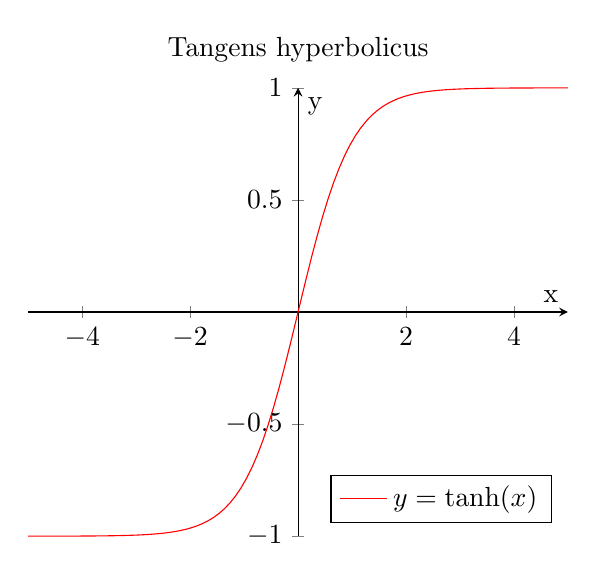
\begin{tikzpicture}
	\begin{axis}[axis lines = center, title={Tangens hyperbolicus},xlabel={x},ylabel={y}, xmin=-5, xmax=5, ymin=-1, ymax=1, grid style=minor, legend pos = south east]
	\addplot[domain=-5:5, samples=100, color=red]{tanh(x)};
	\legend{$y = \tanh(x)$}
	\end{axis}
	\end{tikzpicture}
	\caption{Funktionsgraph des Tangens hyperbolicus}\label{fig:tanh_function}
\end{figure}
In dieser Arbeit konnten die besseren Lernergebnisse unter Verwendung des Tangens hyperbolicus erzielt werden.
\section{Gradient Descent}
Grundidee von Neuronalen Netzen ist, das Netz mit Hilfe von Trainigsdatensätzen auf die Erkennung von Mustern zu trainieren. Eine Menge an Eingangsdaten erzeugt eine Menge an Ist-Ausgabedaten, welche eine Differenz zu gegebenen Soll-Ausgabedaten aufweist. Im Fall der in dieser Arbeit behandelten Erkennung von handschriftlichen Ziffern besteht die Eingabemenge aus einem $28\times28$-Pixel großen Eingabebild und die Ausgabemenge aus einer zehn Werte umfassenden Zuordnung der Eingabe zu der dargestellten Ziffer. Die Pixel des Eingabebildes werden in Graustufen im Intervall $[0;1]$ angegeben, um den Anforderungen der Neuronen zu genügen. In der geordneten Ausgabemenge, ist jeder der möglichen Ziffern genau ein Wert zugeordnet. Stellt die Eingabe die betreffende Ziffer dar, so ist der zugeordnete Ausgabewert $1$, andernfalls $0$. \par Das Neuronale Netz berechnet dementsprechend zehn Ausgabewerte, welche als Wahrscheinlichkeit für das Vorhandensein der jeweiligen Ziffer in der Eingabe gesehen werden kann. Somit kann für jeden Ausgabewerte eine Abweichung zum Sollwert bestimmt werden. Um nun eine Aussage über die Qualität Ausgabebestimmung des Netzes zu einem gegebenen Eingabebild in der momentanen Konfiguration von Gewichten $w$ und Biases $b$ zu bestimmen, muss eine Kostenfunktion definiert werden (vgl. \cite{NNADL_cost_1}). In dieser Arbeit wurde dazu die Kreuzentropie, im weiteren Verlauf auch als Cross Entropy bezeichnet, als Kostenfunktion $C(w,b)$ verwendet. Dabei sind die Funktionsparameter zu beachten. Die Kostenfunktion von Neuronalen Netzen beschreiben im Allgemeinen eine Funktion von Gewichten $w$ und Biases $b$. \par 
Die Allgemeine Form der Kreuzentropie stellt eine Funktion $H(p,q)$ von zwei Wahrscheinlichkeitsverteilungen $p(x)$ und $q(x)$ dar.
\begin{align}
	H(p,q) = - \sum_{x} p(x)\log q(x)
\end{align}
Im Fall des hier beschriebenen Neuronalen Netzes ist die Cross-Entropy-Kostenfunktion $C_E(w,b)$ wie in Gleichung \ref{eq:cross_entropy} dargestellt definiert.
\begin{align}
	C_E(w,b) = - \sum_{i=0}^{9} y_i\log x_i \label{eq:cross_entropy}
\end{align}
Dabei stellt $y_i$ den gegebenen Sollwert für eine mögliche Ziffer dar und $x_i$ die zugehörige berechnete Wahrscheinlichkeit. Eindeutiges Ziel des Trainings des Netzes ist es offensichtlich diese Kostenfunktion zu minimieren. Eine Minimierung der Kosten bedeutet eine genauere Abbildung der Eingabemenge auf das korrekte Ausgabeergebnis. \par Mit Hilfe des Gradienten $\nabla C_E$ kann nun bestimmt werden in welcher Weise die Gewichte $w$ und die Biases $b$ verändert werden müssen, um ein besseres Ergebnis zu erzielen. Der Gradient $\nabla C_E$ ist dabei wie ein Gleichung \ref{eq:nabla_c} definiert.
\begin{align}
	\nabla C_E = \begin{pmatrix}
	\frac{\partial C_E}{\partial w} \\
	\frac{\partial C_E}{\partial b}
	\end{pmatrix} \label{eq:nabla_c}
\end{align} 
Die Änderung der Kosten $\Delta C_E(w,b)$ bestimmt sich bei kleinen Änderungen der Gewichte $\Delta w$ und kleinen Änderungen der Biases $\Delta b$ nach Gleichung \ref{eq:delta_c}.
\begin{align}
	\Delta C_E = \frac{\partial C_E}{\partial w}\Delta w + \frac{\partial C_E}{\partial b}\Delta b \label{eq:delta_c}
\end{align}
Wenn nun die partiellen Ableitungen $\frac{\partial C_E}{\partial w}$ und $\frac{\partial C_E}{\partial b}$ bestimmt werden, können die Kosten in kleinen Schritten dem Kostenminimum angenähert werden. Die Schrittweiten $\Delta w$ und $\Delta b$ werden in Neuronalen Netzen über die \emph{Learning Rate $\eta$} bestimmt. Dieser Parameter bestimmt die Geschwindigkeit des Lernprozesses. Er sollte aber gering gehalten werden, da bei großen $\eta$ ein Pendeln um das Kostenminimum entstehen kann. Die Learning Rate kann im Laufe des Lernprozesses auch dynamisch angepasst bzw. verringert werden um das Lernen zu beschleunigen und im späteren Verlauf des Lernprozesses die Genauigkeit der Anpassung zu erhöhen. \\
\paragraph{Stochastic Gradient Descent}
Um die Gesamtkosten des Lernprozesses zu bestimmen, muss das Neuronale Netz die Outputs aller Bilder des kompletten Trainingsdatensatzes bestimmen und die Kosten aller einzelnen Muster berechnen und summieren. Danach kann aus den gemittelten Kosten der Gradient $\nabla C(w,b)$ ermittelt werden. Bei großen Datensätzen wie dem hier verwendeten MNIST-Datensatz führt das zu einem langsamen Lernprozess, da der Datensatz komplett durchlaufen werden muss, bis eine Anpassung der Gewichte vorgenommen werden kann. Generell sind sehr viele Anpassungsschritte nötig, um hohe Genauigkeiten des Netzwerks zu erreichen. Eine Lösung für dieses Problem bietet der \emph{Stochastic Gradient Descent}-Ansatz. \par 
Bei Stochastic Gradient Descent nähert man den Gradienten $\nabla C(w,b)$ des Datensatzes über eine Teilmenge dessen an. Diese Teilmenge wird im Folgenden Batch genannt. Die Annahme hinter diesem Ansatz ist, dass in einem zufällig verteilten Batch der Gradient $\nabla C_j(w,b)$ eine Näherung des tatsächlichen Gradient $\nabla C(w,b)$ darstellt (vgl. \cite{NNADL_SGD_1}). 
\begin{align}\label{eq:sgd}
	\nabla C = \frac{\sum_{i=0}^{N}\nabla C_i}{N} \approx \frac{\sum_{k=0}^{M}\nabla {C_j}_k}{M} = \nabla C_j
\end{align}
Gleichung \ref{eq:sgd} zeigt diesen Zusammenhang. Dabei stellt $N$ die Gesamtzahl der Trainingsdaten und $M$ die Größe eines Batches dar. Der Index $j$ bezeichnet das jeweils vorliegende Batch. Verfolgt man nun diesen Ansatz, werden die Gewichte $w$ und Biases $b$ während des Durchlaufens des Trainingsdatensatzes mehrmals angepasst und der Lernprozess des Neuronalen Netzes wird deutlich beschleunigt. 
\section{Backpropagation} \label{sec:backpropagation}
Im Jahr 1986 stellten David E. Rumelhart, Geoffrey E. Hinton und Ronald J. Williams in ihrem Paper \emph{Learning representations by back-propagating errors} den Algorithmus zur hier beschriebenen Backpropagation vor. Mit Hilfe dieser Methodik kann ein Zusammenhang zwischen der Änderung der Kostenfunktion $\nabla C(w,b)$, welche nur im finalen Layer exakt bestimmt werden kann, und den Änderungen der Gewichte $\Delta w$ und Biases $\Delta b$ der einzelnen Neuronen im gesamten Netz hergestellt werden. Dadurch wird es möglich, aus den Kosten $\nabla C(w,b)$ alle Gewichte $w$ und Biases $b$ im Netz anzupassen. \par 
Der Backpropagation-Algorithmus basiert auf der Erkenntnis, dass zwischen dem Output jedes Neurons ein linearer Zusammenhang mit den Neuronen der vorhergehenden Schicht besteht (vgl. \cite{BACKPROP_1986}). Es wird nun angenommen, jedem Neuron im Netzwerk wird eine Änderung $\Delta z$ zugewiesen, wobei \begin{align}\label{eq:def_z}z = w\cdot x + b\end{align} definiert wird. Des Weiteren wird ein $\delta_i$ für jedes Neuron nach Gleichung \ref{eq:def_delta} definiert.
\begin{align}
	\delta_i = \frac{\partial C}{\partial z_i} \label{eq:def_delta}
\end{align}
Der Backpropagation-Algorithmus stellt nun ein Verfahren zur Verfügung, welches dieses $\delta_i$ aus den Neuronen der finalen Schicht $L$ für alle Neuronen des Netzwerks rückwirkend bestimmt. Die $\delta_j^L$ der letzten Schicht können nach Gleichung \ref{eq:delta_L} bestimmt werden.
\begin{align}
	\delta_j^L = \frac{\partial C}{\partial o_j^L}\sigma'(z_j^L) \label{eq:delta_L}
\end{align}
Dabei stellt $o_j = \sigma(z_j)$ den Output eines Neurons $j$ dar. Die $\delta_j^l$ der weiteren Schichten $l$ können nacheinander über Gleichung \ref{eq:delta_l} bestimmt werden.
\begin{align}
	\delta^l = ((w^{l+1})^T\delta^{l+1}) \circ \sigma'(z^l) \label{eq:delta_l}
\end{align}
Hierbei beschreibt der Operator $\circ$ das Hadamard-Produkt, welches die elementweise Multiplikation von Vektoren beschreibt. In Gleichung \ref{eq:delta_l} beschreiben $\delta^l$ und $z^l$ jeweils die Vektoren für die zugehörigen Schichten $l$ und $w^{l+1}$ die Matrix der Gewichte zwischen den Schichten $l$ und $(l+1)$. Aufgrund der Linearität von $z$ lassen sich nun über die $delta^l$ die partiellen Ableitungen der Kosten nach den Gewichten $w$ und Biases $b$ bestimmen.
\begin{align}\label{eq:bp4}
	\frac{\partial C}{\partial w^l} &= a^{l-1}\delta^l \\[12pt]\label{eq:bp3}
	\frac{\partial C}{\partial b^l} &= \delta^l 
\end{align}
Mit Hilfe der Gleichungen \ref{eq:delta_L}, \ref{eq:delta_l}, \ref{eq:bp4} und \ref{eq:bp4} lassen sich nun die partiellen Ableitungen der Kosten $C$ nach den Gewichten $w$ und Biases $b$ für jedes Neuron im Netzwerk berechnen. Damit lassen sich durch die Learning Rate $\eta$ alle Gewichte und Biases des Netzwerks anpassen. Somit wird ein Lernprozess durch den Backpropagation-Algorithmus gewährleistet.

\end{document}